\documentclass{standalone}

\usepackage{tikz}
\usepackage{standalone}
\usetikzlibrary{calc}

\begin{document}

    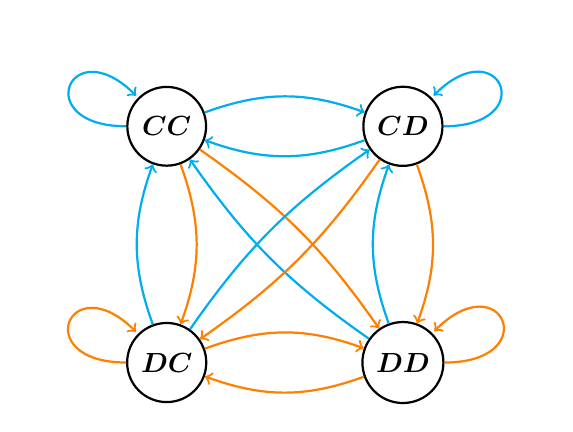
\begin{tikzpicture}

    \tikzstyle{state}=[minimum width=1cm, font=\boldmath];
    

	\node[circle, draw, thick] (0) at (0, 0) [state] {$CC$};
	\node[circle, draw, thick] (1) at (3, 0) [state] {$CD$};
	\node[circle, draw, thick] (2) at (0, -3) [state] {$DC$};
	\node[circle, draw, thick] (3) at (3, -3) [state] {$DD$};

	\draw (0) edge[cyan,out=20, in=160, ->, thick] node [above] {} (1);
	\draw (1) edge[cyan, out=-160, in=-20, ->, thick] node [above] {} (0);

	\draw (2) edge[orange,out=20, in=160, ->, thick] node [above] {} (3);
	\draw (3) edge[orange, out=-160, in=-20, ->, thick] node [above] {} (2);

	\draw (0) edge[orange,out=-70, in=70, ->, thick] node [above] {} (2);
	\draw (2) edge[cyan, out=110, in=-110, ->, thick] node [above] {} (0);

	\draw (1) edge[orange,out=-70, in=70, ->, thick] node [above] {} (3);
	\draw (3) edge[cyan, out=110, in=-110, ->, thick] node [above] {} (1);

    \draw (0) edge[orange,out=-35, in=125, ->, thick] node [above] {} (3);
    \draw (3) edge[cyan, out=145, in=-55, ->, thick] node [above] {} (0);

    \draw (1) edge[orange,out=-125, in=35, ->, thick] node [above] {} (2);
    \draw (2) edge[cyan, out=55, in=-145, ->, thick] node [above] {} (1);

    \draw (0) edge[cyan, out=180, in=135, ->, thick, loop] node [above] {}  (0);
    \draw (2) edge[orange,out=180, in=135, ->, thick, loop] node [above] {} (2);

    \draw (1) edge[cyan,out=0, in=45, ->, thick, loop] node [above] {} (1);
    \draw (3) edge[orange, out=0, in=45, ->, thick, loop] node [above] {} (3);

    \end{tikzpicture}

\end{document}